\newcommand{\downloaderTagResultsAucTable}{
    \begin{table}[h!]
        \centering
        \begin{tabular}{|p{2,8cm}||P{2,2cm} P{2,2cm} P{2,2cm} P{2,2cm}|}
            \hline
            Downloader Tag & ALOHA\newline (M/B only) & ALOHA & Joint\newline Embedding & Proposed\newline Model \\
            \hline
            AUC-ROC & - & 0.973$\pm$0.003 & \textBF{0.977$\pm$0.002} & 0.975$\pm$0.003 \\
            \hline
        \end{tabular}
        \caption[Downloader Tag prediction task AUC-ROC results]{AUC-ROC (Area Under Curve) of the different models for the \textbf{Downloader Tag} prediction task. Results were aggregated over \textBF{3} training runs with different weight initializations and minibatch orderings. Best results are shown in \textbf{bold}.} \label{tab:downloaderTag_auc}
    \end{table}
}

\newcommand{\downloaderTagResultsAtFprTable}{
    \begin{center}
        \begin{longtable}[c]{|P{3,2cm}||P{1,8cm} P{1,8cm} P{1,8cm} P{1,8cm} P{1,8cm}|}
            \hline
            Downloader Tag & \multicolumn{5}{c|}{{FPR}} \\
            & $10^{-5}$ & $10^{-4}$ & $10^{-3}$ & $10^{-2}$ & $10^{-1}$ \\
            \hline
            \endfirsthead

            \caption*{\raggedright ...continued from previous page} \\
            \hline
            Downloader Tag & \multicolumn{5}{c|}{\textbf{FPR}} \\
            & $10^{-5}$ & $10^{-4}$ & $10^{-3}$ & $10^{-2}$ & $10^{-1}$ \\
            \hline
            \endhead

            \caption*{\raggedleft ...continued on next page} \\
            \endfoot

            \caption[Downloader Tag prediction task results]{Mean and standard deviation results (TPR, Accuracy, Recall, Precision and F1-Score) of the different models for the \textbf{Downloader Tag} prediction task at different \textbf{FPR}s (\textit{False Positive Rates}). Results were aggregated over \textBF{3} training runs with different weight initializations and minibatch orderings. Best results are shown in \textbf{bold}. Under \textbf{TPR} results are also presented the percentage reduction in mean detection error and in ROC curve standard deviation introduced by the \textit{Proposed Model} with respect to both \textit{ALOHA} model and \textit{Joint Embedding}.} \label{tab:downloaderTag_results_at_fpr} \\
            \endlastfoot

            \multicolumn{6}{|c|}{\textbf{TPR}} \\
            \hline
            ALOHA (M/B only) & - & - & - & - & - \\
            ALOHA & \textBF{0.227$\pm$0.103} & \textBF{0.439$\pm$0.061} & \textBF{0.550$\pm$0.045} & 0.619$\pm$0.020 & 0.942$\pm$0.002 \\
            Joint Embedding & 0.130$\pm$0.031 & 0.296$\pm$0.071 & 0.543$\pm$0.044 & \textBF{0.638$\pm$0.008} & 0.957$\pm$0.003 \\
            Proposed Model & 0.030$\pm$0.034 & 0.330$\pm$0.067 & 0.530$\pm$0.047 & 0.638$\pm$0.019 & \textBF{0.957$\pm$0.001} \\
            \hline
            Error Reduction wrt\newline ALOHA (M/B only) & - & - & - & - & - \\
            Error Reduction wrt\newline ALOHA & -25.5\% & -19.4\% & -4.4\% & 5.0\% & 25.9\% \\
            Error Reduction wrt\newline Joint Embedding & -11.5\% & 4.8\% & -2.8\% & 0.0\% & 0.0\% \\
            \hline
            Std Reduction wrt\newline ALOHA (M/B only) & - & - & - & - & - \\
            Std Reduction wrt\newline ALOHA & 67.0\% & -9.8\% & -4.4\% & 5.0\% & 50.0\% \\
            Std Reduction wrt\newline Joint Embedding & -9.7\% & 5.6\% & -6.8\% & -137.5\% & 66.7\% \\
            \hline
            \multicolumn{6}{|c|}{\textbf{Accuracy}} \\
            \hline
            ALOHA (M/B only) & - & - & - & - & - \\
            ALOHA & \textBF{0.935$\pm$0.009} & \textBF{0.953$\pm$0.005} & \textBF{0.961$\pm$0.004} & 0.959$\pm$0.002 & 0.904$\pm$0.000 \\
            Joint Embedding & 0.927$\pm$0.003 & 0.941$\pm$0.006 & \textBF{0.961$\pm$0.004} & \textBF{0.961$\pm$0.001} & \textBF{0.905$\pm$0.000} \\
            Proposed Model & 0.919$\pm$0.003 & 0.944$\pm$0.006 & 0.960$\pm$0.004 & 0.961$\pm$0.002 & \textBF{0.905$\pm$0.000} \\
            \hline
            \multicolumn{6}{|c|}{\textbf{Recall}} \\
            \hline
            ALOHA (M/B only) & - & - & - & - & - \\
            ALOHA & \textBF{0.227$\pm$0.103} & \textBF{0.439$\pm$0.061} & \textBF{0.550$\pm$0.045} & 0.619$\pm$0.020 & 0.942$\pm$0.002 \\
            Joint Embedding & 0.130$\pm$0.031 & 0.296$\pm$0.071 & 0.543$\pm$0.044 & \textBF{0.638$\pm$0.008} & 0.957$\pm$0.003 \\
            Proposed Model & 0.030$\pm$0.033 & 0.330$\pm$0.067 & 0.530$\pm$0.047 & 0.638$\pm$0.019 & \textBF{0.957$\pm$0.001} \\
            \hline
            \multicolumn{6}{|c|}{\textbf{Precision}} \\
            \hline
            ALOHA (M/B only) & - & - & - & - & - \\
            ALOHA & \textBF{0.999$\pm$0.000} & \textBF{0.997$\pm$0.000} & \textBF{0.980$\pm$0.002} & 0.850$\pm$0.004 & 0.462$\pm$0.001 \\
            Joint Embedding & \textBF{0.999$\pm$0.000} & 0.996$\pm$0.001 & \textBF{0.980$\pm$0.002} & \textBF{0.853$\pm$0.002} & 0.466$\pm$0.001 \\
            Proposed Model & 0.999$\pm$0.001 & 0.997$\pm$0.001 & \textBF{0.980$\pm$0.002} & 0.853$\pm$0.004 & \textBF{0.466$\pm$0.000} \\
            \hline
            \multicolumn{6}{|c|}{\textbf{F1 Score}} \\
            \hline
            ALOHA (M/B only) & - & - & - & - & - \\
            ALOHA & \textBF{0.358$\pm$0.146} & \textBF{0.607$\pm$0.061} & \textBF{0.704$\pm$0.037} & 0.716$\pm$0.014 & 0.620$\pm$0.001 \\
            Joint Embedding & 0.229$\pm$0.049 & 0.452$\pm$0.083 & 0.698$\pm$0.037 & \textBF{0.730$\pm$0.006} & 0.627$\pm$0.001 \\
            Proposed Model & 0.057$\pm$0.062 & 0.492$\pm$0.074 & 0.687$\pm$0.040 & 0.730$\pm$0.014 & \textBF{0.627$\pm$0.000} \\
            \hline
        \end{longtable}
    \end{center}
}

\newcommand{\downloaderTagResultsSummaryTable}{
    \begin{table}[h!]
        \centering
        \begin{tabular}{|P{3,2cm}||P{1,8cm} P{1,8cm} P{1,8cm} P{1,8cm} P{1,8cm}|}
            \hline
            \multicolumn{6}{|c|}{Downloader Tag (at FPR $=1\%$)} \\
            \hline
            Model & TPR & Accuracy & Precision & Recall & F1 score \\
            \hline
            ALOHA (M/B only) & - & - & - & - & - \\
            ALOHA & 0.619$\pm$0.020 & 0.959$\pm$0.002 & 0.850$\pm$0.004 & 0.619$\pm$0.020 & 0.716$\pm$0.014 \\
            Joint Embedding & \textBF{0.638$\pm$0.008} & \textBF{0.961$\pm$0.001} & \textBF{0.853$\pm$0.002} & \textBF{0.638$\pm$0.008} & \textBF{0.730$\pm$0.006} \\
            Proposed Model & 0.638$\pm$0.019 & 0.961$\pm$0.002 & 0.853$\pm$0.004 & 0.638$\pm$0.019 & 0.730$\pm$0.014 \\
            \hline
        \end{tabular}
        \caption[Summary of Downloader Tag prediction task results]{Summary of the mean and standard deviation results of the different models for the \textbf{Downloader Tag} prediction task at \textbf{FPR} $=1\%$. Results were aggregated over \textBF{3} training runs with different weight initializations and minibatch orderings. Best results are shown in \textbf{bold}.} \label{tab:downloaderTag_result_summary}
    \end{table}
}

\newcommand{\downloaderTagRocAlohaMB}{
    \begin{figure}[h!]
        \vspace*{-0.5cm}
        \centering
        \includegraphics[width=0.6\textwidth]{./results/downloader_tag_roc_alohaMB.png}
        \vspace*{-0.2cm}
        \caption[Downloader Tag prediction task ALOHA (M/B only) ROC curve]{ROC curve and AUC statistics of \textBF{ALOHA (M/B only)} model for the \textbf{Downloader Tag}. The line represents the \textit{mean} TPR at a given FPR, while the shaded region represents the \textit{standard deviation}. Statistics were computed over \textBF{3} training runs, each with random parameter initialization.}
        \label{fig:downloaderTagRocAlohaMB}
    \end{figure}
}

\newcommand{\downloaderTagRocAloha}{
    \begin{figure}[h!]
        \vspace*{-0.5cm}
        \centering
        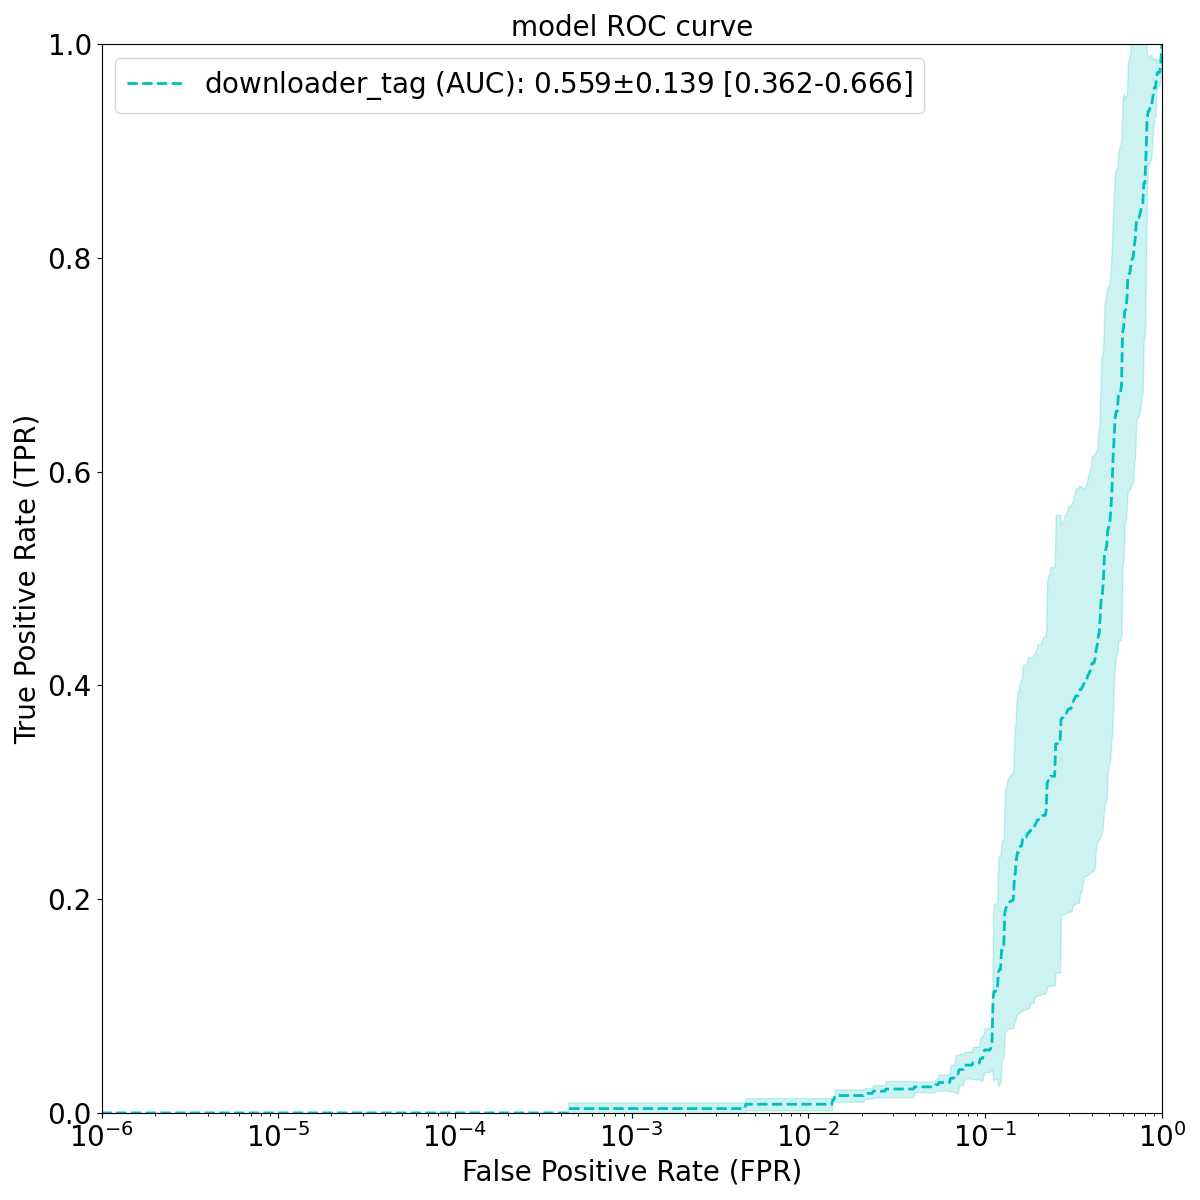
\includegraphics[width=0.6\textwidth]{./results/downloader_tag_roc_aloha.png}
        \vspace*{-0.2cm}
        \caption[Downloader Tag prediction task ALOHA ROC curve]{ROC curve and AUC statistics of \textBF{ALOHA} model for the \textbf{Downloader Tag}. The line represents the \textit{mean} TPR at a given FPR, while the shaded region represents the \textit{standard deviation}. Statistics were computed over \textBF{3} training runs, each with random parameter initialization.}
        \label{fig:downloaderTagRocAloha}
    \end{figure}
}

\newcommand{\downloaderTagRocJointEmbedding}{
    \begin{figure}[h!]
        \vspace*{-0.5cm}
        \centering
        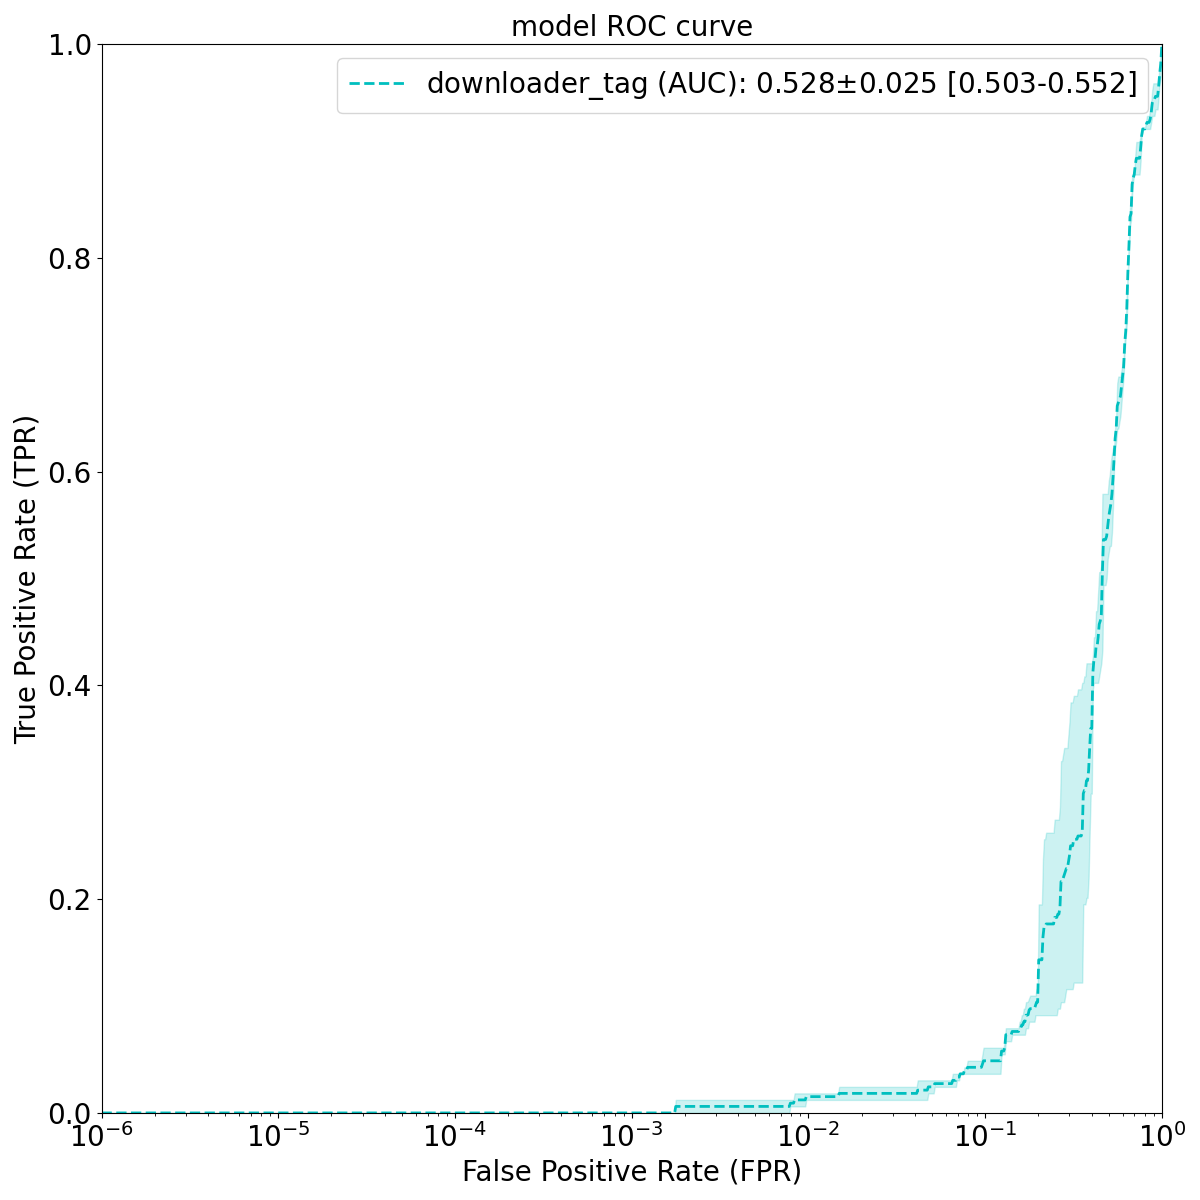
\includegraphics[width=0.6\textwidth]{./results/downloader_tag_roc_jointEmbedding.png}
        \vspace*{-0.2cm}
        \caption[Downloader Tag prediction task Joint Embedding ROC curve]{ROC curve and AUC statistics of \textBF{Joint Embedding} model for the \textbf{Downloader Tag}. The line represents the \textit{mean} TPR at a given FPR, while the shaded region represents the \textit{standard deviation}. Statistics were computed over \textBF{3} training runs, each with random parameter initialization.}
        \label{fig:downloaderTagRocJointEmbedding}
    \end{figure}
}

\newcommand{\downloaderTagRocProposedMethod}{
    \begin{figure}[h!]
        \vspace*{-0.5cm}
        \centering
        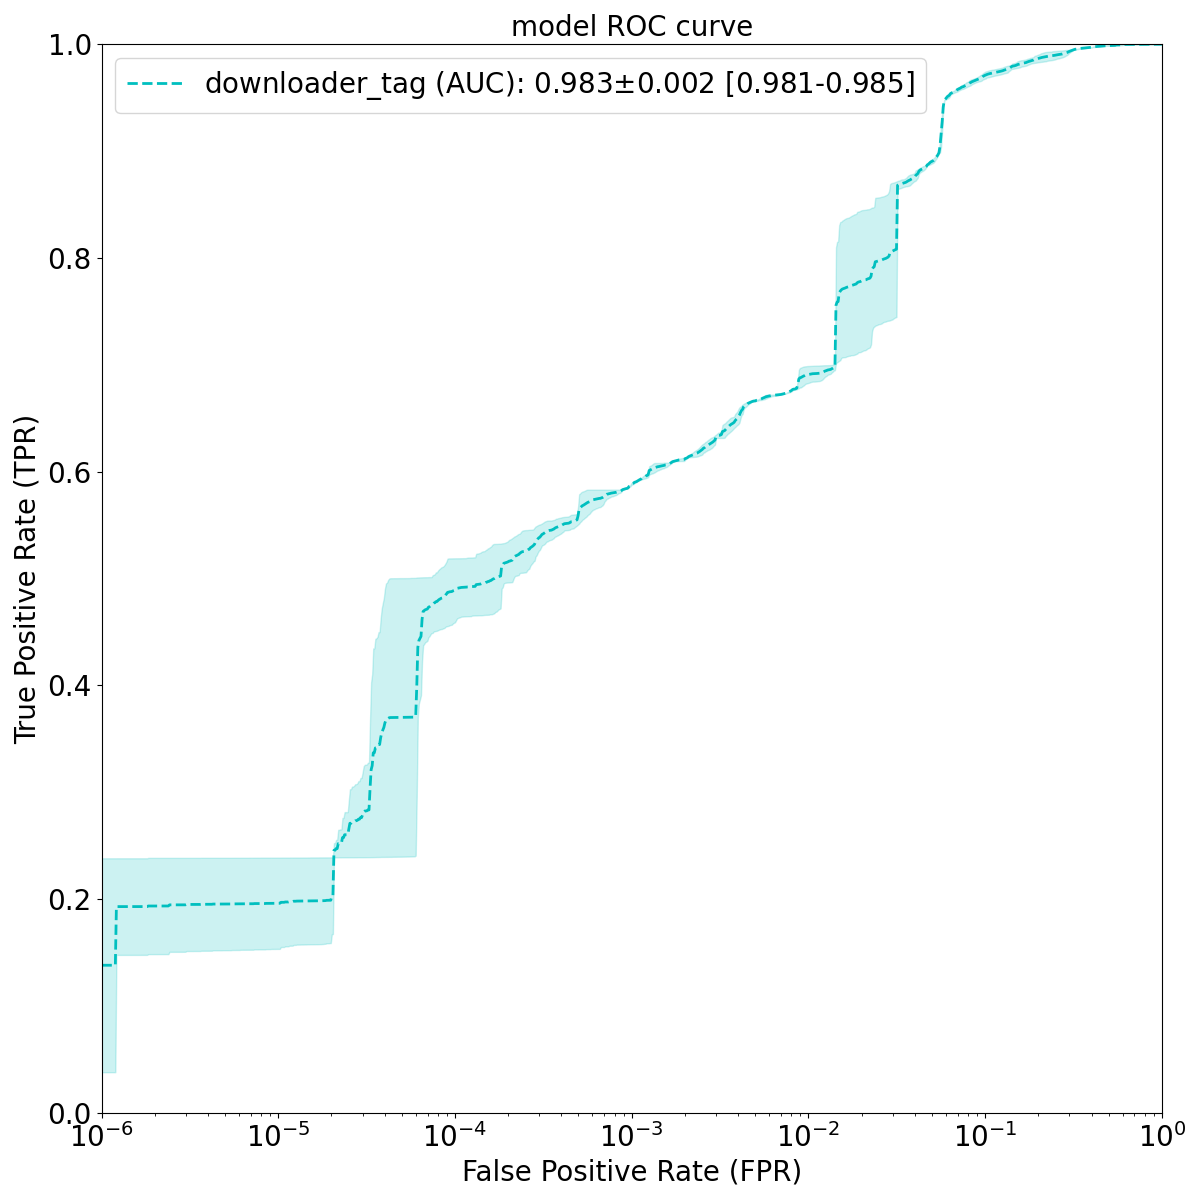
\includegraphics[width=0.6\textwidth]{./results/downloader_tag_roc_proposedModel.png}
        \vspace*{-0.2cm}
        \caption[Downloader Tag prediction task Proposed Model ROC curve]{ROC curve and AUC statistics of \textBF{Proposed Model} for the \textbf{Downloader Tag}. The line represents the \textit{mean} TPR at a given FPR, while the shaded region represents the \textit{standard deviation}. Statistics were computed over \textBF{3} training runs, each with random parameter initialization.}
        \label{fig:downloaderTagRocProposedModel}
    \end{figure}
}
